\documentclass[12pt, twoside]{article}
\usepackage[francais]{babel}
\usepackage[T1]{fontenc}
\usepackage[latin1]{inputenc}
\usepackage[left=5mm, right=5mm, top=3mm, bottom=3mm]{geometry}
\usepackage{float}
\usepackage{graphicx}
\usepackage{array}
\usepackage{multirow}
\usepackage{amsmath,amssymb,mathrsfs} 
\usepackage{soul}
\usepackage{textcomp}
\usepackage{eurosym}
\usepackage{lscape}
 \usepackage{variations}
\usepackage{tabvar}
 
\pagestyle{empty}

\begin{document}
\begin{center}
\Large{\ul{\textbf{Cosinus d'un angle aigu}}}
\end{center}

\section{Quelques rappels}

\ul{D�finition}: Dans un triangle rectangle, le cosinus d'un angle aigu est le
quotient de la longueur du c�t� adjacent � cet angle par la longueur de
l'hypot�nuse:

\begin{center}
\fbox{cosinus d'un angle aigu =$\dfrac{\text{longueur du c�t� adjacent �
l'angle}}{\text{longueur de l'hypot�nuse}}$}
\end{center}

\enskip

\ul{Remarque}: 
Le cosinus d'un angle aigu est toujours compris entre 0 et 1.


\section{Exemples}

\subsection{Calculer la mesure d'un angle}

\ul{Exemple}: Soit FUN un triangle rectangle en U tel que FN=6cm et UN=4cm.
Calculer la mesure de l'angle $\widehat{UNF}$ arrrondie au degr�.


\begin{center}
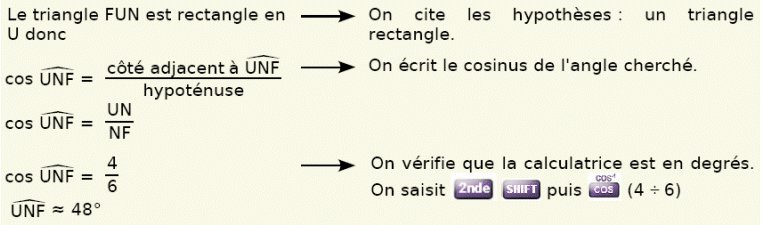
\includegraphics[width=11cm]{images/angle.jpg}
\end{center}



\subsection{Calcul de la longueur du c�t� adjacent � l'angle connu}


\ul{Exemple}: On consid�re un triangle LEA rectangle en E tel que LA=5cm et
$\widehat{ELA}=50$�. 
Calculer la longueur [LE] arrondie au millim�tre.


\begin{center}
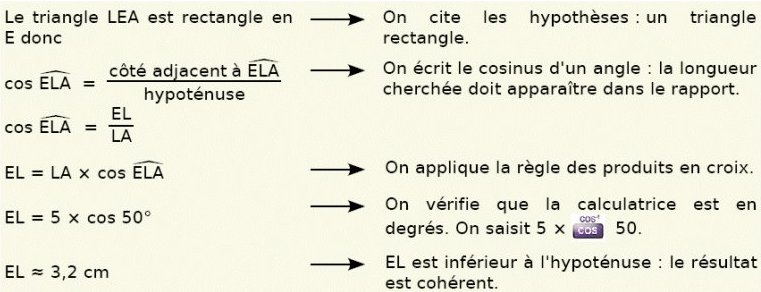
\includegraphics[width=11cm]{images/adjacent.jpg}
\end{center}

\subsection{Calcul de la longueur de l'hypot�nuse}


\ul{Exemple}: On consid�re PAT un triangle rectangle en T tel que AT=7cm et
$\widehat{PAT}=25$�. 
Calculer la longueur [PA] arrondie au millim�tre.

 
\begin{center}
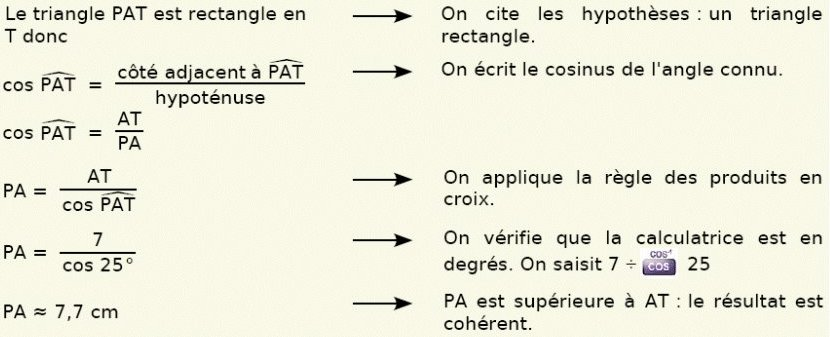
\includegraphics[width=11cm]{images/hypotenuse.jpg}
\end{center}
\end{document}
